\documentclass[11pt,letterpaper]{article}
\usepackage[margin=1in]{geometry}
\usepackage{setspace}      % optional line

\usepackage[T1]{fontenc}
\usepackage[utf8]{inputenc}
\usepackage{lmodern}
\usepackage{microtype}
\usepackage{graphicx}
\usepackage{amsmath}
\usepackage{xcolor}
\usepackage{enumitem}

\begin{document}

\title{Summer Project}
\author{Cyrus Young}
\date{April 10, 2026}


\maketitle

\tableofcontents

\newpage

\section{Background Information}

\subsection{Optical Physics}

The optical beam is modelled as a Gaussian beam propagating along the optical axis ($z$-axis). Working in the paraxial approximation, the complex electric field is
\begin{equation}
    E(x,y,z) = E_0\frac{w_0}{w(z)}\exp\!\left(-\frac{x^2+y^2}{w(z)^2}\right)
    \exp\!\left(-ikz - i\frac{k(x^2+y^2)}{2R(z)} + i\zeta(z)\right),
\end{equation}
where $k = 2\pi/\lambda$ is the wavenumber and the beam parameters are
\begin{align}
    w(z)     &= w_0\sqrt{1+\left(\frac{z}{z_R}\right)^2}, \\
    R(z)     &= z\!\left(1+\left(\frac{z_R}{z}\right)^2\right), \\
    \zeta(z) &= \arctan\!\left(\frac{z}{z_R}\right), \qquad z_R = \frac{\pi w_0^2}{\lambda}.
\end{align}
Here $w_0$ is the beam waist, $w(z)$ is the beam radius at position $z$, $R(z)$ is the radius of curvature of the wavefronts, $\zeta(z)$ is the Gouy phase, and $z_R$ is the Rayleigh range.

At the SLM plane $z=z_0$ the amplitude prefactor $w_0/w(z_0)$ is constant, and $\exp(-ikz_0)$ and $\exp(i\zeta(z_0))$ are \emph{global} phases, so they may be dropped. The curvature term
\[
\exp\!\left(-i\frac{k(x^2+y^2)}{2R(z_0)}\right)
\]
is spatially varying and should be retained unless the beam is well collimated. The incident field at the SLM plane is therefore
\begin{equation}
    E_{\mathrm{in}}(x,y) = A\exp\!\left(-\frac{x^2+y^2}{w^2}\right)
    \exp\!\left(-i\frac{k(x^2+y^2)}{2R}\right),
\end{equation}
where $w \equiv w(z_0)$, $R \equiv R(z_0)$, and $A$ absorbs all constant prefactors. In the collimated limit ($R\to\infty$) this reduces to
\begin{equation}
    E_{\mathrm{in}}(x,y) = A\exp\!\left(-\frac{x^2+y^2}{w^2}\right).
\end{equation}

The modulated field then propagates through thermo-optical material modelled by a linear
transmission matrix $T$, and the detector measures only intensity:
\begin{equation}
    E_{\mathrm{out}} = T\,E_{\mathrm{SLM}}, \qquad I(x,y) = \left|E_{\mathrm{out}}(x,y)\right|^2.
\end{equation}

Optical detectors measure intensity, not complex amplitude, so $I(x,y)$ is the
only accessible quantity.

In summary, the incident field is the Gaussian beam evaluated at the SLM plane; spatially
varying curvature phase is retained when needed; the downstream optical medium is captured
by a complex transmission matrix; and the output camera measures intensity.

\subsection{Thermal Physics}

The optical medium is treated as a thermally perturbed phase/scattering element whose temperature
field evolves on timescales much slower than the optical field. Over these slower thermal timescales,
the temperature distribution \(T(\mathbf{r},t)\) is modelled by the heat equation
\begin{equation}
\rho c_p \frac{\partial T}{\partial t}
=
\nabla \cdot (\kappa \nabla T) + Q(\mathbf{r},t),
\end{equation}
where \(\rho\) is the density, \(c_p\) is the specific heat capacity, \(\kappa\) is the thermal conductivity,
and \(Q(\mathbf{r},t)\) is any applied or absorbed heat source.

Temperature affects the optical response through the thermo-optic effect. To first order, the
refractive index is taken to vary linearly with temperature:
\begin{equation}
n(\mathbf{r},t)=n_0+\frac{dn}{dT}\bigl(T(\mathbf{r},t)-T_0\bigr),
\end{equation}
where \(n_0\) is the reference refractive index at temperature \(T_0\), and \(dn/dT\) is the
thermo-optic coefficient of the material. These refractive-index variations change the optical path
length through the medium and therefore introduce a time-dependent phase perturbation
\begin{equation}
\Delta \phi(x,y,t)=k\int \Delta n(x,y,z,t)\,dz,
\end{equation}
with \(k=2\pi/\lambda\) and \(\Delta n = n-n_0\).

At the system level, these thermally induced phase changes are represented as a slow drift in the
effective optical operator of the medium. In the transmission-matrix description used here, this is
written as

\begin{equation}
T_{\mathrm{opt}}(t)=T_{\mathrm{opt},0}+\Delta T_{\mathrm{opt}}(t),
\end{equation}
where \(T_{\mathrm{opt},0}\) is the nominal transmission matrix and \(\Delta T_{\mathrm{opt}}(t)\) captures the
time-varying perturbation caused by thermal diffusion. The key thermal-physics problem is therefore
to model how heat input produces a temperature field, how that temperature field modifies refractive
index, and how the resulting refractive-index changes alter the optical response seen by the detector.

\subsection{SLM Behaviour}

The SLM acts only in the transverse $(x,y)$ plane and is modeled as a phase-only modulator. The
applied phase pattern $\phi(x,y)$ is the control input and sets the relative phases across the
aperture, thereby altering interference at the output. The modulated field is
\[
E_{\mathrm{SLM}}(x,y)=E_{\mathrm{in}}(x,y)e^{i\phi(x,y)}.
\]

\subsection{Physics-Informed Neural Networks}

Physics-informed neural networks (PINNs) are a class of neural-network models in which the unknown
solution of a physical system is represented by a trainable function and constrained not only by data,
but also by the governing differential equations of the system. Rather than learning an arbitrary
input--output map, a PINN seeks a function that is consistent with both observations and the known
underlying physics.

In the present context, the relevant unknown field is the temperature distribution
\(T(\mathbf{r},t)\) inside the thermo-optical material. A PINN represents this field by a neural
network \(T_\theta(\mathbf{r},t)\), where \(\theta\) denotes the trainable parameters. The network is
then trained so that its output satisfies the heat equation
\begin{equation}
\rho c_p \frac{\partial T_\theta}{\partial t}
-
\nabla \cdot (\kappa \nabla T_\theta)
-
Q(\mathbf{r},t)
= 0
\end{equation}
at a set of collocation points in space and time, while also matching any available initial conditions,
boundary conditions, and measurement data.

The training objective therefore consists of several terms. A typical PINN loss takes the form
\begin{equation}
\mathcal{L}
=
\lambda_{\mathrm{data}}\mathcal{L}_{\mathrm{data}}
+
\lambda_{\mathrm{PDE}}\mathcal{L}_{\mathrm{PDE}}
+
\lambda_{\mathrm{BC}}\mathcal{L}_{\mathrm{BC}}
+
\lambda_{\mathrm{IC}}\mathcal{L}_{\mathrm{IC}},
\end{equation}
where \(\mathcal{L}_{\mathrm{data}}\) penalizes disagreement with observed data,
\(\mathcal{L}_{\mathrm{PDE}}\) penalizes violations of the governing heat equation,
\(\mathcal{L}_{\mathrm{BC}}\) enforces boundary conditions, and
\(\mathcal{L}_{\mathrm{IC}}\) enforces the initial temperature field. The PDE residual is evaluated
using automatic differentiation, which allows spatial and temporal derivatives of the neural-network
output to be computed directly during training.

Once a thermally consistent approximation \(T_\theta(\mathbf{r},t)\) has been learned, it can be
coupled to the optical model through the thermo-optic relation
\begin{equation}
n_\theta(\mathbf{r},t)
=
n_0+\frac{dn}{dT}\bigl(T_\theta(\mathbf{r},t)-T_0\bigr),
\end{equation}
which gives a corresponding refractive-index field. This refractive-index variation induces a
time-dependent optical phase perturbation,
\begin{equation}
\Delta \phi_\theta(x,y,t)
=
k\int \bigl(n_\theta(x,y,z,t)-n_0\bigr)\,dz,
\end{equation}
and hence modifies the effective optical response of the medium. In this way, the PINN serves as a
physics-constrained surrogate model for the thermal dynamics that drive drift in the optical system.

The main advantage of this approach is that it embeds known thermal physics directly into the learning
process, reducing the need for large volumes of labelled data and producing predictions that remain
consistent with the governing equations. For the present project, this provides a principled framework
for learning the slow time evolution of the thermo-optical material and relating that evolution to the
changing interference pattern observed at the detector.


\newpage

\section{Experimental Setup}

A setup of our system is shown below in Figure~\ref{fig:setup}.

\begin{figure}[ht]
    \centering
    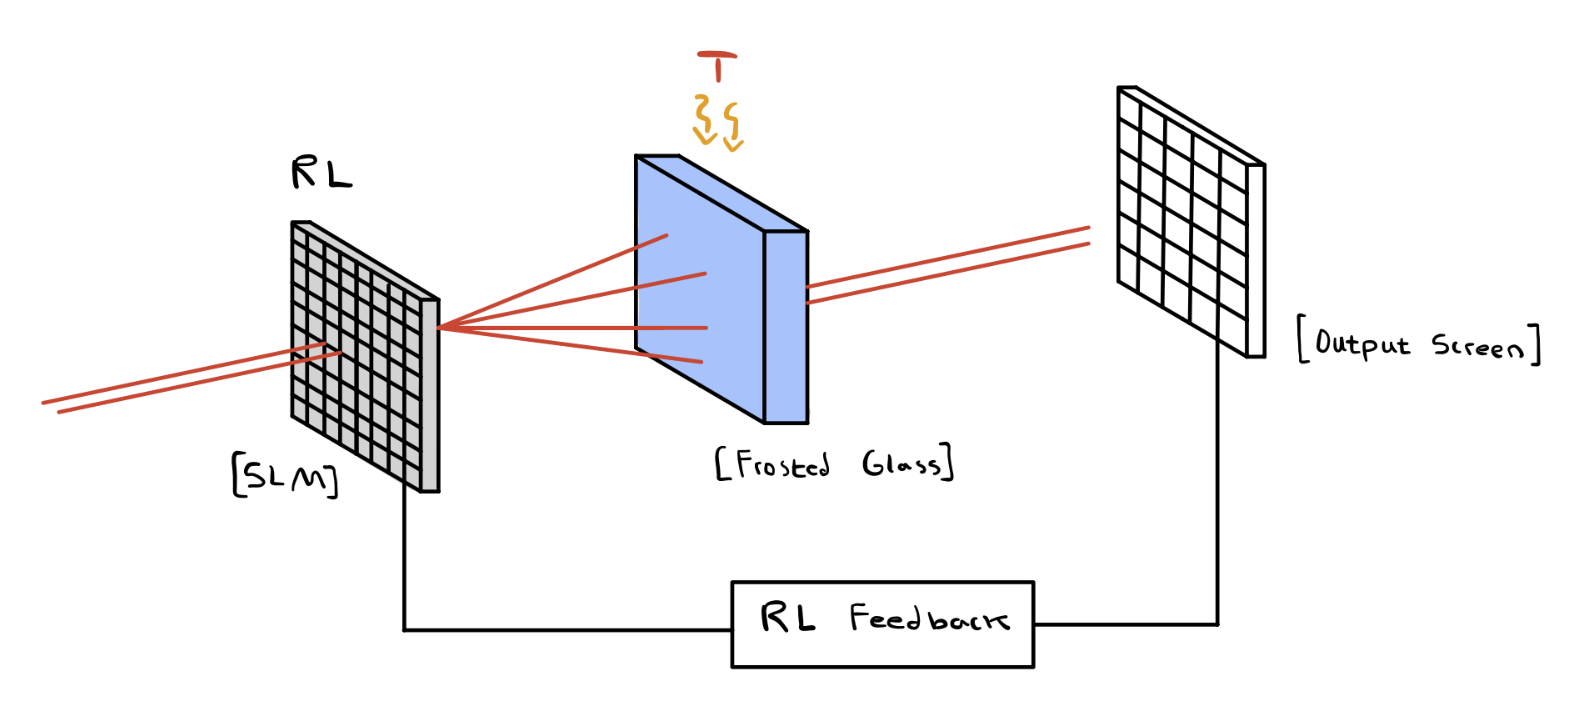
\includegraphics[width=0.7\textwidth]{figures/setup.png}
    \caption{Schematic of the experimental setup. The laser beam is modulated by the SLM, passes through the some material, and is detected by the camera.}
    \label{fig:setup}
\end{figure}
The optical process is summarized as follows:


\begin{enumerate}[label=\textcolor{blue}{\roman*}.]
    \item Define the incident field $E_{\mathrm{in}}(x,y)$ at the SLM plane.
    \item Apply SLM phase modulation to obtain $E_{\mathrm{SLM}}(x,y)=E_{\mathrm{in}}(x,y)e^{i\phi(x,y)}$.
    \item Propagate through the thermo-optical material using the transmission matrix $T_{\mathrm{opt}}(t)$ to give $E_{\mathrm{out}}=T_{\mathrm{opt}}(t)E_{\mathrm{SLM}}$.
    \item Compute the output intensity $I(x,y)=|E_{\mathrm{out}}(x,y)|^2$.
    \item Define the reinforcement-learning reward as the intensity at a selected target output location.
\end{enumerate}

\end{document}
